\documentclass[12pt]{article}

%packages
%\usepackage{latexsym}
\usepackage{graphicx}
\usepackage{color}
\usepackage{amsmath}
\usepackage{dsfont}
\usepackage{placeins}
\usepackage{amssymb}
\usepackage{wasysym}
\usepackage{abstract}
\usepackage{hyperref}
\usepackage{etoolbox}
\usepackage{datetime}
\usepackage{xcolor}
\usepackage{alphalph}
\settimeformat{ampmtime}

%\usepackage{pstricks,pst-node,pst-tree}

%\usepackage{algpseudocode}
%\usepackage{amsthm}
%\usepackage{hyperref}
%\usepackage{mathrsfs}
%\usepackage{amsfonts}
%\usepackage{bbding}
%\usepackage{listings}
%\usepackage{appendix}
\usepackage[margin=1in]{geometry}
%\geometry{papersize={8.5in,11in},total={6.5in,9in}}
%\usepackage{cancel}
%\usepackage{algorithmic, algorithm}

\makeatletter
\def\maxwidth{ %
  \ifdim\Gin@nat@width>\linewidth
    \linewidth
  \else
    \Gin@nat@width
  \fi
}
\makeatother

\definecolor{fgcolor}{rgb}{0.345, 0.345, 0.345}
\newcommand{\hlnum}[1]{\textcolor[rgb]{0.686,0.059,0.569}{#1}}%
\newcommand{\hlstr}[1]{\textcolor[rgb]{0.192,0.494,0.8}{#1}}%
\newcommand{\hlcom}[1]{\textcolor[rgb]{0.678,0.584,0.686}{\textit{#1}}}%
\newcommand{\hlopt}[1]{\textcolor[rgb]{0,0,0}{#1}}%
\newcommand{\hlstd}[1]{\textcolor[rgb]{0.345,0.345,0.345}{#1}}%
\newcommand{\hlkwa}[1]{\textcolor[rgb]{0.161,0.373,0.58}{\textbf{#1}}}%
\newcommand{\hlkwb}[1]{\textcolor[rgb]{0.69,0.353,0.396}{#1}}%
\newcommand{\hlkwc}[1]{\textcolor[rgb]{0.333,0.667,0.333}{#1}}%
\newcommand{\hlkwd}[1]{\textcolor[rgb]{0.737,0.353,0.396}{\textbf{#1}}}%

\usepackage{framed}
\makeatletter
\newenvironment{kframe}{%
 \def\at@end@of@kframe{}%
 \ifinner\ifhmode%
  \def\at@end@of@kframe{\end{minipage}}%
  \begin{minipage}{\columnwidth}%
 \fi\fi%
 \def\FrameCommand##1{\hskip\@totalleftmargin \hskip-\fboxsep
 \colorbox{shadecolor}{##1}\hskip-\fboxsep
     % There is no \\@totalrightmargin, so:
     \hskip-\linewidth \hskip-\@totalleftmargin \hskip\columnwidth}%
 \MakeFramed {\advance\hsize-\width
   \@totalleftmargin\z@ \linewidth\hsize
   \@setminipage}}%
 {\par\unskip\endMakeFramed%
 \at@end@of@kframe}
\makeatother

\definecolor{shadecolor}{rgb}{.77, .77, .77}
\definecolor{messagecolor}{rgb}{0, 0, 0}
\definecolor{warningcolor}{rgb}{1, 0, 1}
\definecolor{errorcolor}{rgb}{1, 0, 0}
\newenvironment{knitrout}{}{} % an empty environment to be redefined in TeX

\usepackage{alltt}
\usepackage[T1]{fontenc}

\newcommand{\qu}[1]{``#1''}
\newcounter{probnum}
\setcounter{probnum}{1}

%create definition to allow local margin changes
\def\changemargin#1#2{\list{}{\rightmargin#2\leftmargin#1}\item[]}
\let\endchangemargin=\endlist 

%allow equations to span multiple pages
\allowdisplaybreaks

%define colors and color typesetting conveniences
\definecolor{gray}{rgb}{0.5,0.5,0.5}
\definecolor{black}{rgb}{0,0,0}
\definecolor{white}{rgb}{1,1,1}
\definecolor{blue}{rgb}{0.5,0.5,1}
\newcommand{\inblue}[1]{\color{blue}#1 \color{black}}
\definecolor{green}{rgb}{0.133,0.545,0.133}
\newcommand{\ingreen}[1]{\color{green}#1 \color{black}}
\definecolor{yellow}{rgb}{1,1,0}
\newcommand{\inyellow}[1]{\color{yellow}#1 \color{black}}
\definecolor{orange}{rgb}{0.9,0.649,0}
\newcommand{\inorange}[1]{\color{orange}#1 \color{black}}
\definecolor{red}{rgb}{1,0.133,0.133}
\newcommand{\inred}[1]{\color{red}#1 \color{black}}
\definecolor{purple}{rgb}{0.58,0,0.827}
\newcommand{\inpurple}[1]{\color{purple}#1 \color{black}}
\definecolor{backgcode}{rgb}{0.97,0.97,0.8}
\definecolor{Brown}{cmyk}{0,0.81,1,0.60}
\definecolor{OliveGreen}{cmyk}{0.64,0,0.95,0.40}
\definecolor{CadetBlue}{cmyk}{0.62,0.57,0.23,0}

%define new math operators
\DeclareMathOperator*{\argmax}{arg\,max~}
\DeclareMathOperator*{\argmin}{arg\,min~}
\DeclareMathOperator*{\argsup}{arg\,sup~}
\DeclareMathOperator*{\arginf}{arg\,inf~}
\DeclareMathOperator*{\convolution}{\text{\Huge{$\ast$}}}
\newcommand{\infconv}[2]{\convolution^\infty_{#1 = 1} #2}
%true functions

%%%% GENERAL SHORTCUTS

%shortcuts for pure typesetting conveniences
\newcommand{\bv}[1]{\boldsymbol{#1}}

%shortcuts for compound constants
\newcommand{\BetaDistrConst}{\dfrac{\Gamma(\alpha + \beta)}{\Gamma(\alpha)\Gamma(\beta)}}
\newcommand{\NormDistrConst}{\dfrac{1}{\sqrt{2\pi\sigma^2}}}

%shortcuts for conventional symbols
\newcommand{\tsq}{\tau^2}
\newcommand{\tsqh}{\hat{\tau}^2}
\newcommand{\sigsq}{\sigma^2}
\newcommand{\sigsqsq}{\parens{\sigma^2}^2}
\newcommand{\sigsqovern}{\dfrac{\sigsq}{n}}
\newcommand{\tausq}{\tau^2}
\newcommand{\tausqalpha}{\tau^2_\alpha}
\newcommand{\tausqbeta}{\tau^2_\beta}
\newcommand{\tausqsigma}{\tau^2_\sigma}
\newcommand{\betasq}{\beta^2}
\newcommand{\sigsqvec}{\bv{\sigma}^2}
\newcommand{\sigsqhat}{\hat{\sigma}^2}
\newcommand{\sigsqhatmlebayes}{\sigsqhat_{\text{Bayes, MLE}}}
\newcommand{\sigsqhatmle}[1]{\sigsqhat_{#1, \text{MLE}}}
\newcommand{\bSigma}{\bv{\Sigma}}
\newcommand{\bSigmainv}{\bSigma^{-1}}
\newcommand{\thetavec}{\bv{\theta}}
\newcommand{\thetahat}{\hat{\theta}}
\newcommand{\thetahatmle}{\hat{\theta}_{\mathrm{MLE}}}
\newcommand{\thetavechatmle}{\hat{\thetavec}_{\mathrm{MLE}}}
\newcommand{\muhat}{\hat{\mu}}
\newcommand{\musq}{\mu^2}
\newcommand{\muvec}{\bv{\mu}}
\newcommand{\muhatmle}{\muhat_{\text{MLE}}}
\newcommand{\lambdahat}{\hat{\lambda}}
\newcommand{\lambdahatmle}{\lambdahat_{\text{MLE}}}
\newcommand{\etavec}{\bv{\eta}}
\newcommand{\alphavec}{\bv{\alpha}}
\newcommand{\minimaxdec}{\delta^*_{\mathrm{mm}}}
\newcommand{\ybar}{\bar{y}}
\newcommand{\xbar}{\bar{x}}
\newcommand{\Xbar}{\bar{X}}
\newcommand{\phat}{\hat{p}}
\newcommand{\Phat}{\hat{P}}
\newcommand{\Zbar}{\bar{Z}}
\newcommand{\iid}{~{\buildrel iid \over \sim}~}
\newcommand{\inddist}{~{\buildrel ind \over \sim}~}
\newcommand{\approxdist}{~{\buildrel approx \over \sim}~}
\newcommand{\equalsindist}{~{\buildrel d \over =}~}
\newcommand{\loglik}[1]{\ell\parens{#1}}
\newcommand{\thetahatkminone}{\thetahat^{(k-1)}}
\newcommand{\thetahatkplusone}{\thetahat^{(k+1)}}
\newcommand{\thetahatk}{\thetahat^{(k)}}
\newcommand{\half}{\frac{1}{2}}
\newcommand{\third}{\frac{1}{3}}
\newcommand{\twothirds}{\frac{2}{3}}
\newcommand{\fourth}{\frac{1}{4}}
\newcommand{\fifth}{\frac{1}{5}}
\newcommand{\sixth}{\frac{1}{6}}

%shortcuts for vector and matrix notation
\newcommand{\A}{\bv{A}}
\newcommand{\At}{\A^T}
\newcommand{\Ainv}{\inverse{\A}}
\newcommand{\B}{\bv{B}}
\newcommand{\K}{\bv{K}}
\newcommand{\Kt}{\K^T}
\newcommand{\Kinv}{\inverse{K}}
\newcommand{\Kinvt}{(\Kinv)^T}
\newcommand{\M}{\bv{M}}
\newcommand{\Bt}{\B^T}
\newcommand{\Q}{\bv{Q}}
\newcommand{\Qt}{\Q^T}
\newcommand{\R}{\bv{R}}
\newcommand{\Rt}{\R^T}
\newcommand{\Z}{\bv{Z}}
\newcommand{\X}{\bv{X}}
\renewcommand{\H}{\bv{H}}
\newcommand{\Xsub}{\X_{\text{(sub)}}}
\newcommand{\Xsubadj}{\X_{\text{(sub,adj)}}}
\newcommand{\I}{\bv{I}}
\newcommand{\Y}{\bv{Y}}
\newcommand{\sigsqI}{\sigsq\I}
\renewcommand{\P}{\bv{P}}
\newcommand{\Psub}{\P_{\text{(sub)}}}
\newcommand{\Pt}{\P^T}
\newcommand{\Pii}{P_{ii}}
\newcommand{\Pij}{P_{ij}}
\newcommand{\IminP}{(\I-\P)}
\newcommand{\Xt}{\bv{X}^T}
\newcommand{\XtX}{\Xt\X}
\newcommand{\XtXinv}{\parens{\Xt\X}^{-1}}
\newcommand{\XtXinvXt}{\XtXinv\Xt}
\newcommand{\XXtXinvXt}{\X\XtXinvXt}
\newcommand{\x}{\bv{x}}
\renewcommand{\b}{\bv{b}}
\newcommand{\onevec}{\bv{1}}
\newcommand{\oneton}{1, \ldots, n}
\newcommand{\yoneton}{y_1, \ldots, y_n}
\newcommand{\yonetonorder}{y_{(1)}, \ldots, y_{(n)}}
\newcommand{\Yoneton}{Y_1, \ldots, Y_n}
\newcommand{\iinoneton}{i \in \braces{\oneton}}
\newcommand{\onetom}{1, \ldots, m}
\newcommand{\jinonetom}{j \in \braces{\onetom}}
\newcommand{\xoneton}{x_1, \ldots, x_n}
\newcommand{\Xoneton}{X_1, \ldots, X_n}
\newcommand{\xt}{\x^T}
\newcommand{\y}{\bv{y}}
\newcommand{\yt}{\y^T}
\renewcommand{\c}{\bv{c}}
\newcommand{\ct}{\c^T}
\newcommand{\tstar}{\bv{t}^*}
\renewcommand{\u}{\bv{u}}
\renewcommand{\v}{\bv{v}}
\renewcommand{\a}{\bv{a}}
\newcommand{\s}{\bv{s}}
\newcommand{\yadj}{\y_{\text{(adj)}}}
\newcommand{\xjadj}{\x_{j\text{(adj)}}}
\newcommand{\xjadjM}{\x_{j \perp M}}
\newcommand{\yhat}{\hat{\y}}
\newcommand{\yhatsub}{\yhat_{\text{(sub)}}}
\newcommand{\yhatstar}{\yhat^*}
\newcommand{\yhatstarnew}{\yhatstar_{\text{new}}}
\newcommand{\z}{\bv{z}}
\newcommand{\zt}{\z^T}
\newcommand{\bb}{\bv{b}}
\newcommand{\bbt}{\bb^T}
\newcommand{\bbeta}{\bv{\beta}}
\newcommand{\beps}{\bv{\epsilon}}
\newcommand{\bepst}{\beps^T}
\newcommand{\e}{\bv{e}}
\newcommand{\Mofy}{\M(\y)}
\newcommand{\KofAlpha}{K(\alpha)}
\newcommand{\ellset}{\mathcal{L}}
\newcommand{\oneminalph}{1-\alpha}
\newcommand{\SSE}{\text{SSE}}
\newcommand{\SSEsub}{\text{SSE}_{\text{(sub)}}}
\newcommand{\MSE}{\text{MSE}}
\newcommand{\RMSE}{\text{RMSE}}
\newcommand{\SSR}{\text{SSR}}
\newcommand{\SST}{\text{SST}}
\newcommand{\JSest}{\delta_{\text{JS}}(\x)}
\newcommand{\Bayesest}{\delta_{\text{Bayes}}(\x)}
\newcommand{\EmpBayesest}{\delta_{\text{EmpBayes}}(\x)}
\newcommand{\BLUPest}{\delta_{\text{BLUP}}}
\newcommand{\MLEest}[1]{\hat{#1}_{\text{MLE}}}

%shortcuts for Linear Algebra stuff (i.e. vectors and matrices)
\newcommand{\twovec}[2]{\bracks{\begin{array}{c} #1 \\ #2 \end{array}}}
\newcommand{\threevec}[3]{\bracks{\begin{array}{c} #1 \\ #2 \\ #3 \end{array}}}
\newcommand{\fivevec}[5]{\bracks{\begin{array}{c} #1 \\ #2 \\ #3 \\ #4 \\ #5 \end{array}}}
\newcommand{\twobytwomat}[4]{\bracks{\begin{array}{cc} #1 & #2 \\ #3 & #4 \end{array}}}
\newcommand{\threebytwomat}[6]{\bracks{\begin{array}{cc} #1 & #2 \\ #3 & #4 \\ #5 & #6 \end{array}}}

%shortcuts for conventional compound symbols
\newcommand{\thetainthetas}{\theta \in \Theta}
\newcommand{\reals}{\mathbb{R}}
\newcommand{\complexes}{\mathbb{C}}
\newcommand{\rationals}{\mathbb{Q}}
\newcommand{\integers}{\mathbb{Z}}
\newcommand{\naturals}{\mathbb{N}}
\newcommand{\forallninN}{~~\forall n \in \naturals}
\newcommand{\forallxinN}[1]{~~\forall #1 \in \reals}
\newcommand{\matrixdims}[2]{\in \reals^{\,#1 \times #2}}
\newcommand{\inRn}[1]{\in \reals^{\,#1}}
\newcommand{\mathimplies}{\quad\Rightarrow\quad}
\newcommand{\mathlogicequiv}{\quad\Leftrightarrow\quad}
\newcommand{\eqncomment}[1]{\quad \text{(#1)}}
\newcommand{\limitn}{\lim_{n \rightarrow \infty}}
\newcommand{\limitN}{\lim_{N \rightarrow \infty}}
\newcommand{\limitd}{\lim_{d \rightarrow \infty}}
\newcommand{\limitt}{\lim_{t \rightarrow \infty}}
\newcommand{\limitsupn}{\limsup_{n \rightarrow \infty}~}
\newcommand{\limitinfn}{\liminf_{n \rightarrow \infty}~}
\newcommand{\limitk}{\lim_{k \rightarrow \infty}}
\newcommand{\limsupn}{\limsup_{n \rightarrow \infty}}
\newcommand{\limsupk}{\limsup_{k \rightarrow \infty}}
\newcommand{\floor}[1]{\left\lfloor #1 \right\rfloor}
\newcommand{\ceil}[1]{\left\lceil #1 \right\rceil}

%shortcuts for environments
\newcommand{\beqn}{\vspace{-0.25cm}\begin{eqnarray*}}
\newcommand{\eeqn}{\end{eqnarray*}}
\newcommand{\bneqn}{\vspace{-0.25cm}\begin{eqnarray}}
\newcommand{\eneqn}{\end{eqnarray}}

%shortcuts for mini environments
\newcommand{\parens}[1]{\left(#1\right)}
\newcommand{\squared}[1]{\parens{#1}^2}
\newcommand{\tothepow}[2]{\parens{#1}^{#2}}
\newcommand{\prob}[1]{\mathbb{P}\parens{#1}}
\newcommand{\cprob}[2]{\prob{#1~|~#2}}
\newcommand{\littleo}[1]{o\parens{#1}}
\newcommand{\bigo}[1]{O\parens{#1}}
\newcommand{\Lp}[1]{\mathbb{L}^{#1}}
\renewcommand{\arcsin}[1]{\text{arcsin}\parens{#1}}
\newcommand{\prodonen}[2]{\bracks{\prod_{#1=1}^n #2}}
\newcommand{\mysum}[4]{\sum_{#1=#2}^{#3} #4}
\newcommand{\sumonen}[2]{\sum_{#1=1}^n #2}
\newcommand{\infsum}[2]{\sum_{#1=1}^\infty #2}
\newcommand{\infprod}[2]{\prod_{#1=1}^\infty #2}
\newcommand{\infunion}[2]{\bigcup_{#1=1}^\infty #2}
\newcommand{\infinter}[2]{\bigcap_{#1=1}^\infty #2}
\newcommand{\infintegral}[2]{\int^\infty_{-\infty} #2 ~\text{d}#1}
\newcommand{\supthetas}[1]{\sup_{\thetainthetas}\braces{#1}}
\newcommand{\bracks}[1]{\left[#1\right]}
\newcommand{\braces}[1]{\left\{#1\right\}}
\newcommand{\set}[1]{\left\{#1\right\}}
\newcommand{\abss}[1]{\left|#1\right|}
\newcommand{\norm}[1]{\left|\left|#1\right|\right|}
\newcommand{\normsq}[1]{\norm{#1}^2}
\newcommand{\inverse}[1]{\parens{#1}^{-1}}
\newcommand{\rowof}[2]{\parens{#1}_{#2\cdot}}

%shortcuts for functionals
\newcommand{\realcomp}[1]{\text{Re}\bracks{#1}}
\newcommand{\imagcomp}[1]{\text{Im}\bracks{#1}}
\newcommand{\range}[1]{\text{range}\bracks{#1}}
\newcommand{\colsp}[1]{\text{colsp}\bracks{#1}}
\newcommand{\rowsp}[1]{\text{rowsp}\bracks{#1}}
\newcommand{\tr}[1]{\text{tr}\bracks{#1}}
\newcommand{\rank}[1]{\text{rank}\bracks{#1}}
\newcommand{\proj}[2]{\text{Proj}_{#1}\bracks{#2}}
\newcommand{\projcolspX}[1]{\text{Proj}_{\colsp{\X}}\bracks{#1}}
\newcommand{\median}[1]{\text{median}\bracks{#1}}
\newcommand{\mean}[1]{\text{mean}\bracks{#1}}
\newcommand{\dime}[1]{\text{dim}\bracks{#1}}
\renewcommand{\det}[1]{\text{det}\bracks{#1}}
\newcommand{\expe}[1]{\mathbb{E}\bracks{#1}}
\newcommand{\expeabs}[1]{\expe{\abss{#1}}}
\newcommand{\expesub}[2]{\mathbb{E}_{#1}\bracks{#2}}
\newcommand{\indic}[1]{\mathds{1}_{#1}}
\newcommand{\var}[1]{\mathbb{V}\text{ar}\bracks{#1}}
\newcommand{\cov}[2]{\mathbb{C}\text{ov}\bracks{#1, #2}}
\newcommand{\corr}[2]{\text{Corr}\bracks{#1, #2}}
\newcommand{\se}[1]{\mathbb{S}\text{E}\bracks{#1}}
\newcommand{\seest}[1]{\hat{\mathbb{S}\text{E}}\bracks{#1}}
\newcommand{\bias}[1]{\text{Bias}\bracks{#1}}
\newcommand{\derivop}[2]{\dfrac{\text{d}}{\text{d} #1}\bracks{#2}}
\newcommand{\partialop}[2]{\dfrac{\partial}{\partial #1}\bracks{#2}}
\newcommand{\secpartialop}[2]{\dfrac{\partial^2}{\partial #1^2}\bracks{#2}}
\newcommand{\mixpartialop}[3]{\dfrac{\partial^2}{\partial #1 \partial #2}\bracks{#3}}

%shortcuts for functions
\renewcommand{\exp}[1]{\mathrm{exp}\parens{#1}}
\renewcommand{\cos}[1]{\text{cos}\parens{#1}}
\renewcommand{\sin}[1]{\text{sin}\parens{#1}}
\newcommand{\sign}[1]{\text{sign}\parens{#1}}
\newcommand{\are}[1]{\mathrm{ARE}\parens{#1}}
\newcommand{\natlog}[1]{\ln\parens{#1}}
\newcommand{\oneover}[1]{\frac{1}{#1}}
\newcommand{\overtwo}[1]{\frac{#1}{2}}
\newcommand{\overn}[1]{\frac{#1}{n}}
\newcommand{\oneoversqrt}[1]{\oneover{\sqrt{#1}}}
\newcommand{\sqd}[1]{\parens{#1}^2}
\newcommand{\loss}[1]{\ell\parens{\theta, #1}}
\newcommand{\losstwo}[2]{\ell\parens{#1, #2}}
\newcommand{\cf}{\phi(t)}

%English language specific shortcuts
\newcommand{\ie}{\textit{i.e.} }
\newcommand{\AKA}{\textit{AKA} }
\renewcommand{\iff}{\textit{iff}}
\newcommand{\eg}{\textit{e.g.} }
\newcommand{\st}{\textit{s.t.} }
\newcommand{\wrt}{\textit{w.r.t.} }
\newcommand{\mathst}{~~\text{\st}~~}
\newcommand{\mathand}{~~\text{and}~~}
\newcommand{\ala}{\textit{a la} }
\newcommand{\ppp}{posterior predictive p-value}
\newcommand{\dd}{dataset-to-dataset}

%shortcuts for distribution titles
\newcommand{\logistic}[2]{\mathrm{Logistic}\parens{#1,\,#2}}
\newcommand{\bernoulli}[1]{\mathrm{Bernoulli}\parens{#1}}
\newcommand{\betanot}[2]{\mathrm{Beta}\parens{#1,\,#2}}
\newcommand{\stdbetanot}{\betanot{\alpha}{\beta}}
\newcommand{\multnormnot}[3]{\mathcal{N}_{#1}\parens{#2,\,#3}}
\newcommand{\normnot}[2]{\mathcal{N}\parens{#1,\,#2}}
\newcommand{\classicnormnot}{\normnot{\mu}{\sigsq}}
\newcommand{\stdnormnot}{\normnot{0}{1}}
\newcommand{\uniformdiscrete}[1]{\mathrm{Uniform}\parens{\braces{#1}}}
\newcommand{\uniform}[2]{\mathrm{U}\parens{#1,\,#2}}
\newcommand{\stduniform}{\uniform{0}{1}}
\newcommand{\geometric}[1]{\mathrm{Geometric}\parens{#1}}
\newcommand{\hypergeometric}[3]{\mathrm{Hypergeometric}\parens{#1,\,#2,\,#3}}
\newcommand{\exponential}[1]{\mathrm{Exp}\parens{#1}}
\newcommand{\gammadist}[2]{\mathrm{Gamma}\parens{#1, #2}}
\newcommand{\poisson}[1]{\mathrm{Poisson}\parens{#1}}
\newcommand{\binomial}[2]{\mathrm{Binomial}\parens{#1,\,#2}}
\newcommand{\negbin}[2]{\mathrm{NegBin}\parens{#1,\,#2}}
\newcommand{\rayleigh}[1]{\mathrm{Rayleigh}\parens{#1}}
\newcommand{\multinomial}[2]{\mathrm{Multinomial}\parens{#1,\,#2}}
\newcommand{\gammanot}[2]{\mathrm{Gamma}\parens{#1,\,#2}}
\newcommand{\cauchynot}[2]{\text{Cauchy}\parens{#1,\,#2}}
\newcommand{\invchisqnot}[1]{\text{Inv}\chisq{#1}}
\newcommand{\invscaledchisqnot}[2]{\text{ScaledInv}\ncchisq{#1}{#2}}
\newcommand{\invgammanot}[2]{\text{InvGamma}\parens{#1,\,#2}}
\newcommand{\chisq}[1]{\chi^2_{#1}}
\newcommand{\ncchisq}[2]{\chi^2_{#1}\parens{#2}}
\newcommand{\ncF}[3]{F_{#1,#2}\parens{#3}}

%shortcuts for PDF's of common distributions
\newcommand{\logisticpdf}[3]{\oneover{#3}\dfrac{\exp{-\dfrac{#1 - #2}{#3}}}{\parens{1+\exp{-\dfrac{#1 - #2}{#3}}}^2}}
\newcommand{\betapdf}[3]{\dfrac{\Gamma(#2 + #3)}{\Gamma(#2)\Gamma(#3)}#1^{#2-1} (1-#1)^{#3-1}}
\newcommand{\normpdf}[3]{\frac{1}{\sqrt{2\pi#3}}\exp{-\frac{1}{2#3}(#1 - #2)^2}}
\newcommand{\normpdfvarone}[2]{\dfrac{1}{\sqrt{2\pi}}e^{-\half(#1 - #2)^2}}
\newcommand{\chisqpdf}[2]{\dfrac{1}{2^{#2/2}\Gamma(#2/2)}\; {#1}^{#2/2-1} e^{-#1/2}}
\newcommand{\invchisqpdf}[2]{\dfrac{2^{-\overtwo{#1}}}{\Gamma(#2/2)}\,{#1}^{-\overtwo{#2}-1}  e^{-\oneover{2 #1}}}
\newcommand{\exponentialpdf}[2]{#2\exp{-#2#1}}
\newcommand{\poissonpdf}[2]{\dfrac{e^{-#1} #1^{#2}}{#2!}}
\newcommand{\binomialpdf}[3]{\binom{#2}{#1}#3^{#1}(1-#3)^{#2-#1}}
\newcommand{\rayleighpdf}[2]{\dfrac{#1}{#2^2}\exp{-\dfrac{#1^2}{2 #2^2}}}
\newcommand{\gammapdf}[3]{\dfrac{#3^#2}{\Gamma\parens{#2}}#1^{#2-1}\exp{-#3 #1}}
\newcommand{\cauchypdf}[3]{\oneover{\pi} \dfrac{#3}{\parens{#1-#2}^2 + #3^2}}
\newcommand{\Gammaf}[1]{\Gamma\parens{#1}}

%shortcuts for miscellaneous typesetting conveniences
\newcommand{\notesref}[1]{\marginpar{\color{gray}\tt #1\color{black}}}

%%%% DOMAIN-SPECIFIC SHORTCUTS

%Real analysis related shortcuts
\newcommand{\zeroonecl}{\bracks{0,1}}
\newcommand{\forallepsgrzero}{\forall \epsilon > 0~~}
\newcommand{\lessthaneps}{< \epsilon}
\newcommand{\fraccomp}[1]{\text{frac}\bracks{#1}}

%Bayesian related shortcuts
\newcommand{\yrep}{y^{\text{rep}}}
\newcommand{\yrepisq}{(\yrep_i)^2}
\newcommand{\yrepvec}{\bv{y}^{\text{rep}}}


%Probability shortcuts
\newcommand{\SigField}{\mathcal{F}}
\newcommand{\ProbMap}{\mathcal{P}}
\newcommand{\probtrinity}{\parens{\Omega, \SigField, \ProbMap}}
\newcommand{\convp}{~{\buildrel p \over \rightarrow}~}
\newcommand{\convLp}[1]{~{\buildrel \Lp{#1} \over \rightarrow}~}
\newcommand{\nconvp}{~{\buildrel p \over \nrightarrow}~}
\newcommand{\convae}{~{\buildrel a.e. \over \longrightarrow}~}
\newcommand{\convau}{~{\buildrel a.u. \over \longrightarrow}~}
\newcommand{\nconvau}{~{\buildrel a.u. \over \nrightarrow}~}
\newcommand{\nconvae}{~{\buildrel a.e. \over \nrightarrow}~}
\newcommand{\convd}{~{\buildrel \mathcal{D} \over \rightarrow}~}
\newcommand{\nconvd}{~{\buildrel \mathcal{D} \over \nrightarrow}~}
\newcommand{\withprob}{~~\text{w.p.}~~}
\newcommand{\io}{~~\text{i.o.}}

\newcommand{\Acl}{\bar{A}}
\newcommand{\ENcl}{\bar{E}_N}
\newcommand{\diam}[1]{\text{diam}\parens{#1}}

\newcommand{\taua}{\tau_a}

\newcommand{\myint}[4]{\int_{#2}^{#3} #4 \,\text{d}#1}
\newcommand{\laplacet}[1]{\mathscr{L}\bracks{#1}}
\newcommand{\laplaceinvt}[1]{\mathscr{L}^{-1}\bracks{#1}}
\renewcommand{\min}[1]{\text{min}\braces{#1}}
\renewcommand{\max}[1]{\text{max}\braces{#1}}

\newcommand{\Vbar}[1]{\bar{V}\parens{#1}}
\newcommand{\expnegrtau}{\exp{-r\tau}}

%%% problem typesetting
\definecolor{darkgrey}{rgb}{0.10,0.10,0.9}

\newcommand{\problem}[1]{\noindent \colorbox{black}{{\color{yellow} \large{\textsf{\textbf{Problem \arabic{probnum}}}}~}} \addtocounter{probnum}{1} \vspace{0.2cm} \\ \iftoggle{professormode}{}{\color{darkgrey}} #1}

\newcommand{\easysubproblem}[1]{\ingreen{\item} \iftoggle{professormode}{}{\color{darkgrey}} [easy] #1 \color{black} }
\newcommand{\intermediatesubproblem}[1]{\inorange{\item} \iftoggle{professormode}{}{\color{darkgrey}} [harder] #1 \color{black} }
\newcommand{\hardsubproblem}[1]{\inred{\item} \iftoggle{professormode}{}{\color{darkgrey}} [difficult] #1 \color{black} }
\newcommand{\extracreditsubproblem}[1]{\inpurple{\item} \iftoggle{professormode}{}{\color{darkgrey}} [E.C.] #1 \color{black} }


\newcommand{\spc}[1]{\iftoggle{professormode}{\\ \vspace{#1cm}}{\\ \vspace{-0.3cm}}}

\makeatletter
\newalphalph{\alphmult}[mult]{\@alph}{26}
\renewcommand{\labelenumi}{(\alphmult{\value{enumi}})}

\newcommand{\support}[1]{\text{Supp}\bracks{#1}}
\newcommand{\mode}[1]{\text{Mode}\bracks{#1}}
\newcommand{\IQR}[1]{\text{IQR}\bracks{#1}}
\newcommand{\quantile}[2]{\text{Quantile}\bracks{#1,\,#2}}


\title{Math 342W / 642 Spring \the\year \\ Midterm Examination Two \inred{Solutions}}
\author{Professor Adam Kapelner}

\date{May 14, \the\year}
\begin{document}
\maketitle

\noindent Full Name \line(1,0){410}

\thispagestyle{empty}

\section*{Code of Academic Integrity}

\footnotesize
Since the college is an academic community, its fundamental purpose is the pursuit of knowledge. Essential to the success of this educational mission is a commitment to the principles of academic integrity. Every member of the college community is responsible for upholding the highest standards of honesty at all times. Students, as members of the community, are also responsible for adhering to the principles and spirit of the following Code of Academic Integrity.

Activities that have the effect or intention of interfering with education, pursuit of knowledge, or fair evaluation of a student's performance are prohibited. Examples of such activities include but are not limited to the following definitions:

\paragraph{Cheating} Using or attempting to use unauthorized assistance, material, or study aids in examinations or other academic work or preventing, or attempting to prevent, another from using authorized assistance, material, or study aids. Example: using an unauthorized cheat sheet in a quiz or exam, altering a graded exam and resubmitting it for a better grade, etc.
\\

\noindent I acknowledge and agree to uphold this Code of Academic Integrity. \\

\begin{center}
\line(1,0){250} ~~~ \line(1,0){100}\\
~~~~~~~~~~~~~~~~~~~~~signature~~~~~~~~~~~~~~~~~~~~~~~~~~~~~~~~~~~~~~~~~~~~~ date
\end{center}

\normalsize
\vspace{-0.5cm}
\section*{Instructions}

This exam is 110 minutes and closed-book. You are allowed \textbf{two} pages (front and back) of a \qu{cheat sheet.} You may use a graphing calculator of your choice. Please read the questions carefully. If the question reads \qu{compute,} this means the solution will be a number otherwise you can leave the answer in \textit{any} widely accepted mathematical notation which could be resolved to an exact or approximate number with the use of a computer. I advise you to skip problems marked \qu{[Extra Credit]} until you have finished the other questions on the exam, then loop back and plug in all the holes. I also advise you to use pencil. The exam score will be normed to be out of 100 points total plus extra credit if it exists. Partial credit will be granted for incomplete answers on most of the questions. \fbox{Box} in your final answers. Good luck!

\pagebreak

\problem In class, we spoke about probability estimation for a binary phenomenon $\mathcal{Y} = \braces{0,1}$. We modeled each observation as an independent $\bernoulli{\theta_i}$ i.e. $Y_i \inddist  \theta_i^{y_i} (1 - \theta_i)^{1-y_i}$ where $\theta_i := \expe{Y_i = 1~|~\x_i}$ which for the Bernoulli is synonymous with $\cprob{Y_i = 1}{\x_i}$ and it varies with observation based on the features $\x_i$ which is a row vector of length $p+1$ since the first entry is set to be one. 

To do so, we used a generalized linear model (GLM) which coerced the linear model $\x \cdot \w$ into the support of the parameter $\theta_i$, a probability ranging from $\bracks{0,1}$. To do this coercion, we used a link function $\phi(\x \cdot \w)$ which mapped $\x \cdot \w \in \reals \rightarrow \support{\theta_i} = \bracks{0,1}$. Any monotonically increasing function with domain $\reals$ and range $\bracks{0,1}$ was legal. For example, any CDF of a random variable with support $\reals$ fits this definition. 

Let's use the link function $\phi(u)$ is the CDF of the standard Gumbel, $F(x) = e^{-e^{-x}}$ where this algorithm is called \qu{cloglog regression} and we'll denote it $\mathcal{A}_{\text{cloglog}}$.

\benum
\subquestionwithpoints{4} Write out the objective function to maximize which is the probability of the entire training set $\mathbb{D}$. Since this is a GLM, your answer must include the linear term for the $i$th observation, $\x_i \cdot \w$. \\

$\cprob{Y_1, \ldots, Y_n}{\x_1, \ldots, \x_n} = \displaystyle\prod_{i=1}^n \cprob{Y_i}{\x_i} =\prod_{i=1}^n \inred{\tothepow{e^{-e^{-\x_i \cdot \w}}}{y_i} \tothepow{1 - e^{-e^{-\x_i \cdot \w}}}{1 - y_i}}  $\\

\subquestionwithpoints{1} Our algorithm $\mathcal{A}_{\text{cloglog}}$ involves running this optimization problem in the computer: $\b := \argmax_{\w} \braces{\text{your answer from the previous problem}}$. What is the dimension of the vector $\b$? ~~\inred{$p+1$}

\subquestionwithpoints{3} Given $\b$ and a new observation $\x_\star$, write the explicit functional form of $g(\x_\star)$, an expression that computes $\hat{p}_\star$, the probability estimate that the measured phenomenon will be one.

\vspace{-0.5cm}
\inred{
\beqn
\hat{p}_\star = e^{-e^{-\x_\star \cdot \b}}
\eeqn
}
We now examine performance of this model out of sample using different $\hat{p}$ thresholds. Here are four of the possible classifiers' oos confusion tables labeled A, B, C, D:


\begin{multicols}{4}
\footnotesize
\setlength{\columnseprule}{0.4pt}
\begin{center}\fbox{A}\end{center}
\begin{verbatim}
      y_test_hat
y_test    0    1
     0 2866  938
     1  144 1052
\end{verbatim}
\inred{
ME = (144+938) / 5000 = 0.216\\
Recall = 1052 / 1196 = 0.88 \\
FPR =  938 / (938 + 2866) = 0.25\\
FP/FN = 938 / 144 = 6.51
}
\columnbreak
\begin{center}\fbox{B}\end{center}
\begin{verbatim}
      y_test_hat
y_test    0    1
     0 3357  447
     1  360  836
\end{verbatim}
\inred{
ME = (447+360) / 5000 = 0.161\\
Recall = 836 / 1196 = 0.70 \\
FPR =  447 / (447 + 3357) = 0.12\\
FP/FN = 447/360 = 1.24
}
\columnbreak
\begin{center}\fbox{C}\end{center}
\begin{verbatim}
      y_test_hat
y_test    0    1
     0 3601  203
     1  611  585
\end{verbatim}
\inred{
ME = (203+611) / 5000 = 0.163\\
Recall = 585 / 1196 = 0.49 \\
FPR =  203 / (203 + 3601) = 0.05\\
FP/FN = 203 / 611 = 0.33
}
\columnbreak
\begin{center}\fbox{D}\end{center}
\begin{verbatim}
      y_test_hat
y_test    0    1
     0 3794   10
     1 1043  153
\end{verbatim}
\inred{
ME = (10+1043) / 5000 = 0.211\\
Recall = 153 / 1196 = 0.13 \\
FPR =  10 / (10 + 3794) = 0.003\\
FP/FN = 10 / 1043 = 0.01
}
\end{multicols}
\pagebreak

%\subquestionwithpoints{6} Assume the dataset now had $p=1$ and $\mathcal{A}_{\text{probit}}$ returned $b_0 = 1.77$ and $b_1 = 1.10$. Interpret the value $b_1 = 1.10$. This means you must write a few sentences in English below.\spc{8}

\subquestionwithpoints{2} With the information provided, is it possible to compute the $\hat{p}$ threshold values for the four classifiers above? Circle one: Yes / \inred{\fbox{No}}


\subquestionwithpoints{1} Which model has the lowest oos misclassification error? Circle one: A / \inred{\fbox{B}} / C / D\spc{-.5}

\subquestionwithpoints{8} Draw the ROC curve below to the best of your ability. Label the axes. Your curve should have 6 include distinct points whose values are marked on the axes. Four of these points should additionally be labeled as A, B, C, D corresponding to the four models displayed on the previous page. 

 
\begin{figure}[htp]
\centering
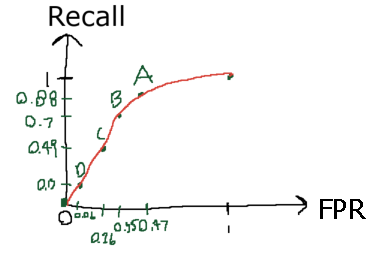
\includegraphics[width=5in]{roc}
\end{figure} 




\subquestionwithpoints{2} Is the oos AUC is definitively greater than 0.5 for this model? Circle one: \inred{\fbox{Yes}} / No\spc{-0.5}

\subquestionwithpoints{2} If false positives were much more costly than false negatives, which one of the four models is best to employ? Circle one: A / B / C / \inred{\fbox{D}}\spc{-0.5}

\subquestionwithpoints{2} If false negatives were much more costly than false positives, which one of the four models is best to employ? Circle one: \inred{\fbox{A}} / B / C / D\spc{-0.5}

\subquestionwithpoints{3} If you required a symmetric-cost classifier, which one out of the four models is best to employ? Circle one: A / \inred{\fbox{B}} / C / D\spc{-0.5}

%Assume $p=1$ for the rest of the problem. Displayed below is $\mathbb{D}_{\text{test}}^\top$ with $n_{\text{test}} = 10$ including the probability estimates from $g$ denoted as the vector $\bv{\hat{p}}$ underneath $\mathbb{D}_{\text{test}}^\top$:
%
%\begin{table}[ht]
%\centering
%\begin{tabular}{r|rrrrrrrrrr}
%$\x_{\cdot 1}$ & -2.51 & 0.73 & -3.34 & 6.38 & 1.32 & -3.28 & 1.95 & 2.95 & 2.30 & -1.22 \\ 
%$\y$ & 1 & 1 & 0 & 1 & 1 & 0 & 1 & 1 & 1 & 0 \\ \hline
%$\bv{\hat{p}}$ & 0.08 & 0.68 & 0.03 & 0.99 & 0.79 & 0.04 & 0.88 & 0.95 & 0.91 & 0.23
%\end{tabular}
%\end{table}~\vspace{1.5cm}
%
%
%\subquestionwithpoints{5} Circle the letters of all the following that are \textbf{true}.
%
%
%\begin{enumerate}[(a)]
%\item You have enough information to compute the out-of-sample Brier scoring rule
%\item You have enough information to compute the out-of-sample log scoring rule
%\item You have enough information to compute the out-of-sample AUC metric
%\item The oos AUC is definiteively greater than 0.5 for this model
%\item You have enough information to compute an approximate out-of-sample DET
%\end{enumerate}
%
%
%\subquestionwithpoints{4} We now use this probit regression model to do binary classification. Using the naive threshold classifier, compute the average oos misclassification error. \spc{2}
%
%\subquestionwithpoints{3} If the cost of false positives was \$2 and the cost of false negatives was \$1, compute an estimate of mean cost per prediction to the nearest cent. \spc{2}
%
%\subquestionwithpoints{4} If the cost of false negatives was much much greater than the cost of false positives, what explicit thresholding rule would minimize mean cost per prediction? Hint: there are many correct answers. \spc{3}

\eenum


%\problem In class, we never spoke about count modeling i.e. $\mathcal{Y} = \braces{0,1, 2, \ldots}$ but it is very similar to our discussion of probability estimation. We will now model each observation as an independent $\poisson{\theta_i}$ i.e. $Y_i \inddist \theta_i^{y_i} e^{-\theta_i} / y_i!$ where $\theta_i$ is the $\expe{Y_i = 1~|~\x_i}$ and it varies with observation based on the features $\x_i$ which is a row vector of length $p+1$ since the first entry is set to be one. 
%
%To do so, we will use a generalized linear model (GLM) which coerces the linear model $\x \cdot \w$ into the support of the parameter $\theta_i$, a mean count ranging in $\parens{0, \infty}$. To do this coercion, we can use a link function $\phi(\x \cdot \w)$ which maps $\x \cdot \w \in \reals \rightarrow \support{\theta_i} = \parens{0, \infty}$. Any monotonically increasing function with domain $\reals$ and range $\parens{0, \infty}$ is legal.
%
%Let's use the link function $\phi(u) = 10^u$. This algorithm is called \qu{poisson regression} and we'll denote it $\mathcal{A}_{\text{poisson}}$.
%
%\benum
%\subquestionwithpoints{6} Write out the objective function to maximize which is the probability of the entire training set $\mathbb{D}$. Since this is a GLM, your answer must include the linear term for the $i$th observation, $\x_i \cdot \w$. \\
%
%$\cprob{Y_1, \ldots, Y_n}{\x_1, \ldots, \x_n} = \displaystyle\prod_{i=1}^n \cprob{Y_i}{\x_i} = \prod_{i=1}^n $\\
%
%\subquestionwithpoints{1} Our algorithm $\mathcal{A}_{\text{poisson}}$ involves running this optimization problem in the computer: $\b := \argmax_{\w} \braces{\text{your answer from the previous problem}}$. What is the dimension of the vector $\b$?
%
%\subquestionwithpoints{4} For the $n_{\text{test}}$ oos responses denoted by the vector $\y$ and oos predictions denoted by the vector $\yhat$, propose a sensical error metric that gauges the oos performance of the model returned by $\mathcal{A}_{\text{poisson}}$. There are many acceptable answers.\spc{3}
%
%\subquestionwithpoints{4} Assume the dataset now had $p=1$ and $\mathcal{A}_{\text{poisson}}$ returned $b_0 = 1.77$ and $b_1 = 1.10$. For $x_\star = 1$, compute $\hat{y}_\star$.\spc{3}
%
%\eenum


\problem In the lab we analyzed three tables: bills and bill payments which have 226,434 rows and 194,850 rows. Here are a subset of interest of the bills table followed by a subset of interest of the bill payments table: \pagebreak

\begin{Verbatim}[frame=single]
         id   due_date invoice_date tot_amount customer_id discount_id
      <num>     <IDat>       <IDat>      <num>       <int>       <num>
 1: 5000000 2016-07-31   2016-06-16   99480.18    12867871     7397895
 2: 5693147 2017-05-11   2017-04-11   99528.76    12871311     7397895
 3: 6098612 2016-01-15   2016-01-04   99477.35    13135347     7397895
 4: 6386294 2016-12-30   2016-12-30   99479.31    12867871     7397895
 5: 6609438 2017-05-07   2017-04-07   99477.20    12867871     7397895
 6: 6791759 2016-12-16   2016-11-16   99477.17    13479284     7397895
 7: 6945910 2017-06-08   2017-06-08   99477.32    12855932     7397895
 8: 7079442 2017-05-12   2017-04-12   99477.19    13135347     7397895
 9: 7197225 2016-05-24   2016-04-24   99485.43    12867871     7397895
10: 7302585 2017-03-28   2017-02-26   99477.47    12855932     7397895

          id paid_amount transaction_date bill_id
       <num>       <num>           <IDat>   <num>
 1: 13780480    99150.43       2016-07-01 5000000
 2: 13654517    99220.42       2016-08-08 5693147
 3:  5000000    99148.07       2016-08-03 6098612
 4: 13845921    99154.67       2016-07-15 6386294
 5:  5693147    99148.07       2016-08-03 6609438
 6:  6945910    99152.35       2016-08-19 7302585
 7:  7197225    99151.47       2016-08-26 7397895
 8:  7079442    99148.43       2016-08-19 7484907
 9:  7302585    99158.61       2016-09-02 7564949
10:  7397895    99148.07       2016-11-04 7890372
\end{Verbatim}

\benum
\subquestionwithpoints{2} If we were to do a left join where the left table was the subset of interest of bills and the right table was the subset of interest of bill payments, what would be the number of rows in the final joined table? \inred{10} 

\subquestionwithpoints{2} Given the join in the previous question, what would be the number of columns in the final joined table? \inred{9}

\subquestionwithpoints{2} Given the join in the previous question, what would be the number of rows in the final joined table after listwise deletion of missingness? \inred{6}

\subquestionwithpoints{3} Consider the table of the subset of interest of bill payments which is in \qu{wide} format. If this table was converted from wide to long format where the metric variables were all variables (except \texttt{id}), how many rows would the final long table have? \inred{30}

\subquestionwithpoints{2} Consider the operation in the previous question. Which table has more entry values? Circle one: \\
~\\
the original wide table / \inred{\fbox{the transformed long table}}






%\subquestionwithpoints{4} If we were to do a left join where the left table was bill discounts and the right table was bills, what would be the minimum number of rows in the final joined table? \spc{1}
%\subquestionwithpoints{2} If we were to do a full join where the left table was bill discounts and the right table was bills, what would be the maximum number of rows in the final joined table? \spc{3}
%
%This page was intentially left blank
%\pagebreak



%\subquestionwithpoints{6} Draw below a long version of the first six rows of the bill discounts table where the metric variables are the columns \texttt{num\_days}, \texttt{pct\_off}, \texttt{days\_until\_discount} and the id column is still the id column. Make sure the long table you display does not have any missingness. Use the listwise deletion procedure to address any missingness if it exists. \spc{9}


%After merging the three tables appropriately, we generated a feature \texttt{paid\_in\_full} $\in \mathcal{Y} = \braces{0,1}$ which will be our prediction target where 1 = the customer indeed paid on time. We also generate reasonable features and drop other columns that have no relevance to our prediction problem. Below is the first 6 rows of the final data frame. The first column is $y$ followed by $p=8$ features.
%
%
%\begin{verbatim}
%   paid_in_full tot_amount num_days_to_pay disc_days discount_pct_off
%1:            0   99505.86               1        13                2
%2:            1   99576.09              30         4               NA
%3:            0   99475.42              30         2               NA
%4:            0   99479.24               1        13                2
%5:            0   99475.05              30        13                2
%6:            0   99475.05              30         4               NA
%   disc_delay num_previous_bills num_prev_bills_yes owed_per_day
%1:         NA                107                  0    99505.857
%2:         NA               4859                922     3319.203
%3:         60               1046                  0     3315.847
%4:         NA               1023                  0    99479.237
%5:         NA                800                  0     3315.835
%6:         NA               1595                860     3315.83
%\end{verbatim}
%
%We then assume the missingness is this data frame is imputed using the missForest algorithm. Assume the final data frame does not have any missingness whatsover.
%
%We then sample 2,000 observations from that final imputed data frame to fit two models of all features on \texttt{paid\_in\_full}:
%
%\begin{enumerate}
%\item[($\mathcal{A} =$ RF)] A random forest classification model with 500 trees, 4 variables tried at each split and nodesize = 400. Here are the OOB results:
%
%\begin{verbatim}
%           predicted 0 predicted 1 model errors
%actual 0          1568         170        0.098
%actual 1            60         202        0.229
%use errors       0.037       0.457        0.115
%  Accuracy: 88.5%
%\end{verbatim}
%
%\item[($\mathcal{A} =$ CART)] A classification tree model with nodesize = 1. Here are the OOB results:
%
%\begin{verbatim} 
%           predicted 0 predicted 1 model errors
%actual 0           614          19        0.030
%actual 1            16          83        0.162
%use errors       0.025       0.186        0.048
%  Accuracy: 95.219%
%\end{verbatim}
%\end{enumerate}
%
%
%\subquestionwithpoints{13} Circle the letters of all the following that are \textbf{true}.
%
%
%\begin{enumerate}[(a)]
%\item The nodesize is a hyperparameter of $\mathcal{A} =$ RF
%\item The nodesize is a hyperparameter of $\mathcal{A} =$ CART
%\item The number of trees is a hyperparameter of $\mathcal{A} =$ RF
%\item The number of trees is a hyperparameter of $\mathcal{A} =$ CART
%\item The number of variables tried at each split is a hyperparameter of $\mathcal{A} =$ RF
%\item The number of variables tried at each split is a hyperparameter of $\mathcal{A} =$ CART
%\item $\mathcal{A} =$ CART cannot overfit since $p=8$ while $n=2,000$
%\item In this example, the CART model is estimated to do better than the RF model when predicting in the future if $c_{FP} = c_{FN}$\\
%
%For the remainder of this true/false set of questions, assume the terms \qu{MSE}, \qu{bias} and \qu{variance} are the terms employed in the bias-variance tradeoff theorem we discussed in class. We will assume that this theorem extends to situations where $\mathcal{Y} = \braces{0,1}$ even though it was proven for $\mathcal{Y} \subseteq \reals$.
%
%\item If the RF model was fit on more than 2,000 observations, it would have had less bias.
%\item If the CART model was fit on more than 2,000 observations, it would have had less bias.
%\item The RF model has less variance than the CART model
%
%\item If the RF model was fit with nodesize = 1, it would have had less bias than the CART model
%\item If the RF model was fit with nodesize = 1, it would have had less variance than the CART model
%\end{enumerate}

%Below is an illustration of tree \#1 in the RF model (fit with 500 trees, 4 variables tried at each split and nodesize = 400). The leaf value of \qu{2.00} means that $\hat{y} = 1$ for that leaf. The left direction mean the inequality in the split rule was true.
%
%\vspace{-0.5cm}
%\begin{figure}[htp]
%\centering
%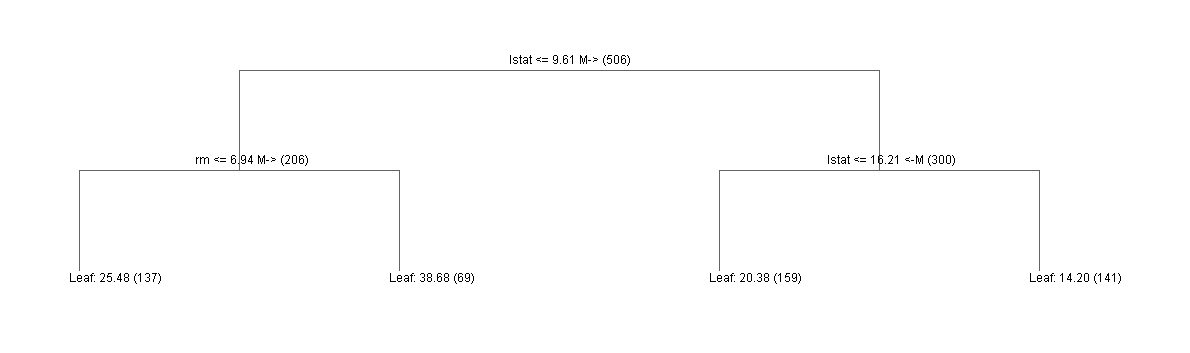
\includegraphics[width=7in]{tree.png}
%\end{figure}
%\vspace{-0.5cm}

\eenum

\problem Consider the following two meta-algorithms: bagging and boosting both with a large number of constituent base learners denoted $M$. Assume the algorithms to generate the \qu{base learners} in both bagging and boosting are the same algorithm denoted $\mathcal{A}$. Let $\mathbb{D}_1 := \angbraces{\X_1, \y_1}, \mathbb{D}_2 := \angbraces{\X_2, \y_2}, \ldots, \mathbb{D}_M := \angbraces{\X_M, \y_M}$ denote the dataset used by each of the base learners. Consider a modeling scenario where $\mathcal{Y} = \reals$ and $f$ is known to be highly non-linear with interactions among the $p$ covariates.

\benum  

\subquestionwithpoints{20} Circle the letters of all the following that are \textbf{true}. 

\begin{enumerate}[(a)]
\item[\inred{\fbox{a}}] In bagging, the higher the $M$, the better the oos performance (in general) 
\item[] In boosting, the higher the $M$, the better the oos performance (in general)

\item[\inred{\fbox{c}}] In bagging, the order of fitting the $M$ base learners does not matter 
\item[] In boosting, the order of fitting the $M$ base learners does not matter

\item[] In bagging at iteration $t$, $\mathbb{D}_t$ is updated with the results of $g_1, g_2, \ldots, g_{t-1}$
\item[\inred{\fbox{f}}] In boosting at iteration $t$, $\mathbb{D}_t$ is updated with the results of $g_1, g_2, \ldots, g_{t-1}$ 

\item[] In bagging, the $M$ base learners are fit on the same dataset i.e. \\ $\mathbb{D}_1 = \mathbb{D}_2 = \ldots = \mathbb{D}_M$
\item[] In boosting, the $M$ base learners are fit on the the same dataset i.e. \\ $\mathbb{D}_1 = \mathbb{D}_2 = \ldots = \mathbb{D}_M$

\item[] In bagging, the $M$ base learners are fit on the the same input matrices i.e. \\ $\X_1 = \X_2 = \ldots = \X_M$
\item[\inred{\fbox{j}}] In boosting, the $M$ base learners are fit on the the same input matrices i.e. \\ $\X_1 = \X_2 = \ldots = \X_M$ 
\item[] In bagging, the $M$ base learners are fit on the the same response vectors i.e. \\ $\y_1 = \y_2 = \ldots = \y_M$ 
\item[] In boosting, the $M$ base learners are fit on the the same response vectors i.e. \\ $\y_1 = \y_2 = \ldots = \y_M$
\item[] In bagging, if $\mathcal{A}$ = OLS, oos performance is likely to be high
\item[] In boosting, if $\mathcal{A}$ = OLS, oos performance is likely to be high
\item[] In bagging, if $\mathcal{A}$ = CART with $N_0$ large, oos performance is likely to be high
\item[\inred{\fbox{p}}] In boosting, if $\mathcal{A}$ = CART with $N_0$ large, oos performance is likely to be high 
\item[\inred{\fbox{q}}] In bagging, if $\mathcal{A}$ = CART with $N_0$ small, oos performance is likely to be high 
\item[] In boosting, if $\mathcal{A}$ = CART with $N_0$ small, oos performance is likely to be high

\item[] Bagging is in general a better meta-algorithm than boosting as measured by oos performance
\item[] Boosting is in general a better meta-algorithm than bagging as measured by oos performance
\end{enumerate}
\pagebreak

\eenum

\problem Consider a subset of the \texttt{boston housing} data frame, which has $n = 500$ observations and $p_{raw} = 13$ numeric measurements. The response variable is \texttt{medv} with an average value of 22.53 (measured in 1000 USD). We wish to fit a forward stepwise OLS model to this data beginning with the intercept and with a pool consisting of all first-order interactions (i.e. the \texttt{R} formula \texttt{y $\sim$ .*.}) 

We split the dataset into a training set of size 300, a select set of size 100 and a test set of size 100. We do not randomize the order of the dataset when doing so. We then use nested resampling which rotates the select set and the test set. Assume we have sufficient resources to run the stepwise until its completion with all first-order interactions for every iteration (in both the inner and outer loops). We report some RMSE metrics below for the first training-select split of the first inner loop:

\begin{Verbatim}[frame=single]
> Dtrain_1_1 = MASS::Boston[1:300, ]
> Dselect_1_1 = MASS::Boston[301:400, ]
> mod_1_1_0 = lm(medv ~ 1, Dtrain_1_1)
> mod_1_1_M = lm(medv ~ . * ., Dtrain_1_1)
> round(summary(mod_1_1_0)$sigma, 2)
[1] 8.89
> round(summary(mod_1_1_M)$sigma, 2)
[1] 2.16
> yhat_1_1_0 = predict(mod_1_1_0, Dselect_1_1)
> sqrt(mean((yhat_1_1_0 - Dselect_1_1$medv)^2))
[1] 10.21488
> yhat_1_1_M = predict(mod_1_1_M, Dselect_1_1)
> sqrt(mean((yhat_1_1_M - Dselect_1_1$medv)^2))
[1] 59.01323
\end{Verbatim}

\benum

\subquestionwithpoints{2} How many different training-select splits are in one inner loop?\\
\inred{$K_{inner} = 4$ since we are dividing 400 observations into a set of 300 and 100.}

\subquestionwithpoints{2} How many different training-test splits are in one outer loop?\\
\inred{$K_{outer} = 5$  since we are dividing 500 observations into a set of 400 and 100.}


\subquestionwithpoints{3} How many iterations of the greedy stepwise algorithm are done for the first training-select split of the first inner loop of the first outer loop?\\~\\
\inred{We begin with the intercept (so that doesn't count as an \qu{iteration}. Then, there's $p$ linear terms, $p$ squared terms and $\binom{p}{2}$ interactions of two different variables, i.e., $ p + p + \binom{p}{2} = 26 + \binom{13}{2} = 104$. Note: addition of the intercept is also accepted as it is ambiguous if it an \qu{iteration} or not. So 105 is the other acceptable answer.}

\subquestionwithpoints{3} How many iterations of the greedy stepwise algorithm are done for the entire nested resampling procedure across all folds?\\~\\
\inred{$\parens{p + p + \binom{p}{2}}K_{inner}K_{outer} = 104(4)(5) = 2080$}

\pagebreak

\subquestionwithpoints{3} When building the final model (after validation is completed), how many iterations of the greedy stepwise algorithm are done across all folds?\\~\\
\inred{$\parens{p + p + \binom{p}{2}}K_{outer} = 104(5) = 520$}


\subquestionwithpoints{5} For the first training-select split of the first inner loop, draw the in-sample RMSE plot as a function degrees of freedom (draw it as best as possible given the information you have). Label your axes and mark critical points numerically.

 
\begin{figure}[htp]
\centering
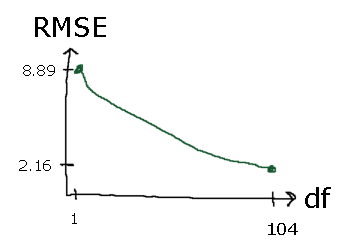
\includegraphics[width=3in]{isRMSE}
\end{figure} 


\subquestionwithpoints{5} For the first training-select split of the first inner loop, draw the oosRMSE plot as a function degrees of freedom (draw it as best as possible given the information you have). Label your axes and mark critical points numerically.


\begin{figure}[htp]
\centering
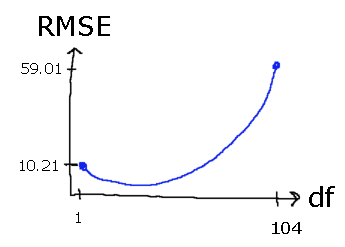
\includegraphics[width=3in]{oosRMSE}
\end{figure} 

We now fit a regression tree to the full boston housing dataset. The full tree model is visualized on the top of the next page.
 
\begin{figure}[htp]
\centering
\hspace*{-2cm}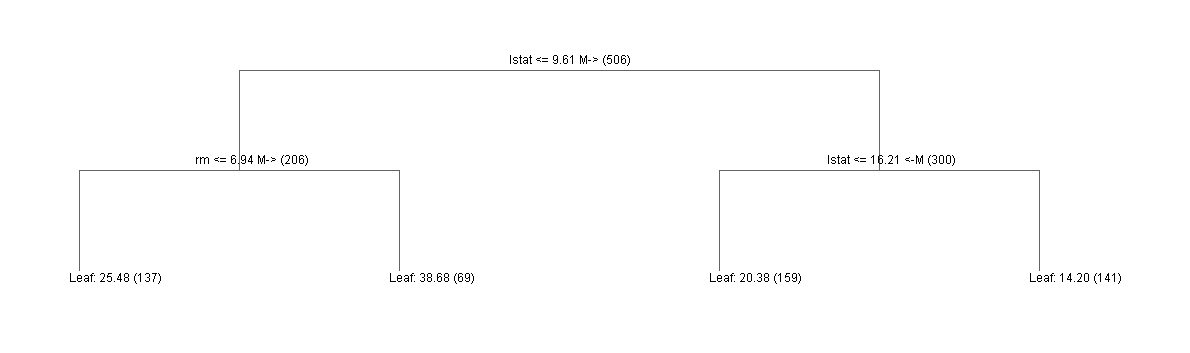
\includegraphics[width=8.2in]{tree.png}
\end{figure} 

\subquestionwithpoints{1} How many nodes does this tree model have?
 \inred{7}
\subquestionwithpoints{2} What are the two most important variables (defined as variables that can decrease in-sample SSE)?
 \inred{lstat, rm}
\subquestionwithpoints{2} What is the most precise statement you can make about the value of $N_0$?
 \inred{$N_0 \geq 159$} 
\pagebreak

\subquestionwithpoints{2} If the same algorithm that produced the tree visualized above was implemented as base learner for bagging with $M$ sufficiently large, would the the oos error of the bagged model be lower than the oos error of the single tree above in all likelihood? Circle one: \inred{\fbox{Yes}} 

\subquestionwithpoints{3} If the same algorithm that produced the tree visualized above was implemented as base learner for random forest with $M$ sufficiently large, what would likely need to be changed about the base learner's algorithm to improve performance?\\ 

\inred{Set $N_0$ to a small value}

\eenum



\problem Assume $g(\x) = \mathcal{A}(\mathbb{D}, \mathcal{H})$ is a model for a real-valued response. In class we studied the following three decompositions of MSE in the modeling context where $\delta$ was realized from a mean-centered r.v. $\Delta$ with variance $\sigsq$ independent of the value of $\x$:

\beqn
&[I]& ~~MSE(\x_*) = \sigsq + (f(\x_*) - g(\x_*))^2 \\
&[II]& ~~MSE(\x_*) = \sigsq + \bias{g(\x_*)}^2 + \var{g(\x_*)} \\
&[III]& ~~MSE = \sigsq + \expe{\bias{g(\x_*)}^2} + \expe{\var{g(\x_*)}} \\
\eeqn

\benum

\subquestionwithpoints{2} In [I], the MSE is taken as an expectation over which random variable(s)? \inred{$\Delta$}

\subquestionwithpoints{3} In [II], the MSE is taken as an expectation over which random variable(s)? \inred{$\Delta, \Y$}

\subquestionwithpoints{3} In [III], the MSE is taken as an expectation over which random variable(s)? \inred{$\Delta, \Y, \X_1, \ldots, \X_n, \X_*$}
\eenum

\end{document}
